% Options for packages loaded elsewhere
% Options for packages loaded elsewhere
\PassOptionsToPackage{unicode}{hyperref}
\PassOptionsToPackage{hyphens}{url}
\PassOptionsToPackage{dvipsnames,svgnames,x11names}{xcolor}
%
\documentclass[
  11pt,
  a4paper,
  DIV=11,
  numbers=noendperiod]{scrartcl}
\usepackage{xcolor}
\usepackage[lmargin=2cm,rmargin=2cm,tmargin=2cm,bmargin=2cm]{geometry}
\usepackage{amsmath,amssymb}
\setcounter{secnumdepth}{-\maxdimen} % remove section numbering
\usepackage{iftex}
\ifPDFTeX
  \usepackage[T1]{fontenc}
  \usepackage[utf8]{inputenc}
  \usepackage{textcomp} % provide euro and other symbols
\else % if luatex or xetex
  \usepackage{unicode-math} % this also loads fontspec
  \defaultfontfeatures{Scale=MatchLowercase}
  \defaultfontfeatures[\rmfamily]{Ligatures=TeX,Scale=1}
\fi
\usepackage{lmodern}
\ifPDFTeX\else
  % xetex/luatex font selection
  \setmainfont[]{Helvetica}
\fi
% Use upquote if available, for straight quotes in verbatim environments
\IfFileExists{upquote.sty}{\usepackage{upquote}}{}
\IfFileExists{microtype.sty}{% use microtype if available
  \usepackage[]{microtype}
  \UseMicrotypeSet[protrusion]{basicmath} % disable protrusion for tt fonts
}{}
\makeatletter
\@ifundefined{KOMAClassName}{% if non-KOMA class
  \IfFileExists{parskip.sty}{%
    \usepackage{parskip}
  }{% else
    \setlength{\parindent}{0pt}
    \setlength{\parskip}{6pt plus 2pt minus 1pt}}
}{% if KOMA class
  \KOMAoptions{parskip=half}}
\makeatother
% Make \paragraph and \subparagraph free-standing
\makeatletter
\ifx\paragraph\undefined\else
  \let\oldparagraph\paragraph
  \renewcommand{\paragraph}{
    \@ifstar
      \xxxParagraphStar
      \xxxParagraphNoStar
  }
  \newcommand{\xxxParagraphStar}[1]{\oldparagraph*{#1}\mbox{}}
  \newcommand{\xxxParagraphNoStar}[1]{\oldparagraph{#1}\mbox{}}
\fi
\ifx\subparagraph\undefined\else
  \let\oldsubparagraph\subparagraph
  \renewcommand{\subparagraph}{
    \@ifstar
      \xxxSubParagraphStar
      \xxxSubParagraphNoStar
  }
  \newcommand{\xxxSubParagraphStar}[1]{\oldsubparagraph*{#1}\mbox{}}
  \newcommand{\xxxSubParagraphNoStar}[1]{\oldsubparagraph{#1}\mbox{}}
\fi
\makeatother

\usepackage{color}
\usepackage{fancyvrb}
\newcommand{\VerbBar}{|}
\newcommand{\VERB}{\Verb[commandchars=\\\{\}]}
\DefineVerbatimEnvironment{Highlighting}{Verbatim}{commandchars=\\\{\}}
% Add ',fontsize=\small' for more characters per line
\usepackage{framed}
\definecolor{shadecolor}{RGB}{241,243,245}
\newenvironment{Shaded}{\begin{snugshade}}{\end{snugshade}}
\newcommand{\AlertTok}[1]{\textcolor[rgb]{0.68,0.00,0.00}{#1}}
\newcommand{\AnnotationTok}[1]{\textcolor[rgb]{0.37,0.37,0.37}{#1}}
\newcommand{\AttributeTok}[1]{\textcolor[rgb]{0.40,0.45,0.13}{#1}}
\newcommand{\BaseNTok}[1]{\textcolor[rgb]{0.68,0.00,0.00}{#1}}
\newcommand{\BuiltInTok}[1]{\textcolor[rgb]{0.00,0.23,0.31}{#1}}
\newcommand{\CharTok}[1]{\textcolor[rgb]{0.13,0.47,0.30}{#1}}
\newcommand{\CommentTok}[1]{\textcolor[rgb]{0.37,0.37,0.37}{#1}}
\newcommand{\CommentVarTok}[1]{\textcolor[rgb]{0.37,0.37,0.37}{\textit{#1}}}
\newcommand{\ConstantTok}[1]{\textcolor[rgb]{0.56,0.35,0.01}{#1}}
\newcommand{\ControlFlowTok}[1]{\textcolor[rgb]{0.00,0.23,0.31}{\textbf{#1}}}
\newcommand{\DataTypeTok}[1]{\textcolor[rgb]{0.68,0.00,0.00}{#1}}
\newcommand{\DecValTok}[1]{\textcolor[rgb]{0.68,0.00,0.00}{#1}}
\newcommand{\DocumentationTok}[1]{\textcolor[rgb]{0.37,0.37,0.37}{\textit{#1}}}
\newcommand{\ErrorTok}[1]{\textcolor[rgb]{0.68,0.00,0.00}{#1}}
\newcommand{\ExtensionTok}[1]{\textcolor[rgb]{0.00,0.23,0.31}{#1}}
\newcommand{\FloatTok}[1]{\textcolor[rgb]{0.68,0.00,0.00}{#1}}
\newcommand{\FunctionTok}[1]{\textcolor[rgb]{0.28,0.35,0.67}{#1}}
\newcommand{\ImportTok}[1]{\textcolor[rgb]{0.00,0.46,0.62}{#1}}
\newcommand{\InformationTok}[1]{\textcolor[rgb]{0.37,0.37,0.37}{#1}}
\newcommand{\KeywordTok}[1]{\textcolor[rgb]{0.00,0.23,0.31}{\textbf{#1}}}
\newcommand{\NormalTok}[1]{\textcolor[rgb]{0.00,0.23,0.31}{#1}}
\newcommand{\OperatorTok}[1]{\textcolor[rgb]{0.37,0.37,0.37}{#1}}
\newcommand{\OtherTok}[1]{\textcolor[rgb]{0.00,0.23,0.31}{#1}}
\newcommand{\PreprocessorTok}[1]{\textcolor[rgb]{0.68,0.00,0.00}{#1}}
\newcommand{\RegionMarkerTok}[1]{\textcolor[rgb]{0.00,0.23,0.31}{#1}}
\newcommand{\SpecialCharTok}[1]{\textcolor[rgb]{0.37,0.37,0.37}{#1}}
\newcommand{\SpecialStringTok}[1]{\textcolor[rgb]{0.13,0.47,0.30}{#1}}
\newcommand{\StringTok}[1]{\textcolor[rgb]{0.13,0.47,0.30}{#1}}
\newcommand{\VariableTok}[1]{\textcolor[rgb]{0.07,0.07,0.07}{#1}}
\newcommand{\VerbatimStringTok}[1]{\textcolor[rgb]{0.13,0.47,0.30}{#1}}
\newcommand{\WarningTok}[1]{\textcolor[rgb]{0.37,0.37,0.37}{\textit{#1}}}

\usepackage{longtable,booktabs,array}
\newcounter{none} % for unnumbered tables
\usepackage{calc} % for calculating minipage widths
% Correct order of tables after \paragraph or \subparagraph
\usepackage{etoolbox}
\makeatletter
\patchcmd\longtable{\par}{\if@noskipsec\mbox{}\fi\par}{}{}
\makeatother
% Allow footnotes in longtable head/foot
\IfFileExists{footnotehyper.sty}{\usepackage{footnotehyper}}{\usepackage{footnote}}
\makesavenoteenv{longtable}
\usepackage{graphicx}
\makeatletter
\newsavebox\pandoc@box
\newcommand*\pandocbounded[1]{% scales image to fit in text height/width
  \sbox\pandoc@box{#1}%
  \Gscale@div\@tempa{\textheight}{\dimexpr\ht\pandoc@box+\dp\pandoc@box\relax}%
  \Gscale@div\@tempb{\linewidth}{\wd\pandoc@box}%
  \ifdim\@tempb\p@<\@tempa\p@\let\@tempa\@tempb\fi% select the smaller of both
  \ifdim\@tempa\p@<\p@\scalebox{\@tempa}{\usebox\pandoc@box}%
  \else\usebox{\pandoc@box}%
  \fi%
}
% Set default figure placement to htbp
\def\fps@figure{htbp}
\makeatother





\setlength{\emergencystretch}{3em} % prevent overfull lines

\providecommand{\tightlist}{%
  \setlength{\itemsep}{0pt}\setlength{\parskip}{0pt}}



 


\KOMAoption{captions}{tableheading}
\makeatletter
\@ifpackageloaded{caption}{}{\usepackage{caption}}
\AtBeginDocument{%
\ifdefined\contentsname
  \renewcommand*\contentsname{Table of contents}
\else
  \newcommand\contentsname{Table of contents}
\fi
\ifdefined\listfigurename
  \renewcommand*\listfigurename{List of Figures}
\else
  \newcommand\listfigurename{List of Figures}
\fi
\ifdefined\listtablename
  \renewcommand*\listtablename{List of Tables}
\else
  \newcommand\listtablename{List of Tables}
\fi
\ifdefined\figurename
  \renewcommand*\figurename{Figure}
\else
  \newcommand\figurename{Figure}
\fi
\ifdefined\tablename
  \renewcommand*\tablename{Table}
\else
  \newcommand\tablename{Table}
\fi
}
\@ifpackageloaded{float}{}{\usepackage{float}}
\floatstyle{ruled}
\@ifundefined{c@chapter}{\newfloat{codelisting}{h}{lop}}{\newfloat{codelisting}{h}{lop}[chapter]}
\floatname{codelisting}{Listing}
\newcommand*\listoflistings{\listof{codelisting}{List of Listings}}
\makeatother
\makeatletter
\makeatother
\makeatletter
\@ifpackageloaded{caption}{}{\usepackage{caption}}
\@ifpackageloaded{subcaption}{}{\usepackage{subcaption}}
\makeatother
\usepackage{bookmark}
\IfFileExists{xurl.sty}{\usepackage{xurl}}{} % add URL line breaks if available
\urlstyle{same}
\hypersetup{
  pdftitle={Data: Team Firefighters},
  pdfauthor={Zeynep Zünbüldere \& Ömer Can Kaynarca},
  colorlinks=true,
  linkcolor={blue},
  filecolor={Maroon},
  citecolor={Blue},
  urlcolor={Blue},
  pdfcreator={LaTeX via pandoc}}


\title{Data: Team Firefighters}
\author{Zeynep Zünbüldere \& Ömer Can Kaynarca}
\date{2026-05-12}
\begin{document}
\maketitle


\section{Data Source \& Our Process}\label{data-source-our-process}

1)In this project, we used 2024 forestry data from OGM to see how
forests are actually spread across Turkey. We wanted to find out which
cities are the greenest and if the results match our common
expectations---like expecting the Mediterranean or Black Sea regions to
have much higher forest density compared to Central Anatolia. To get the
answers, we first imported our Excel file using the readxl package. The
data wasn't perfect at first; we had to clean up extra spaces and remove
total sum rows. A big part of our work was fixing the city names so they
would match our map perfectly---correcting weird typos in the library
like ``Zinguldak'' or ``Kinkkale''.

You can download the final processed dataset here:
\url{proje_verisi.RData}

\#installed the packages with the help of Gemini

\begin{Shaded}
\begin{Highlighting}[]
\FunctionTok{library}\NormalTok{(readxl)}
\FunctionTok{library}\NormalTok{(tidyverse)}
\end{Highlighting}
\end{Shaded}

\begin{verbatim}
-- Attaching core tidyverse packages ------------------------ tidyverse 2.0.0 --
v dplyr     1.2.1     v readr     2.2.0
v forcats   1.0.1     v stringr   1.6.0
v ggplot2   4.0.3     v tibble    3.3.1
v lubridate 1.9.5     v tidyr     1.3.2
v purrr     1.2.2     
-- Conflicts ------------------------------------------ tidyverse_conflicts() --
x dplyr::filter() masks stats::filter()
x dplyr::lag()    masks stats::lag()
i Use the conflicted package (<http://conflicted.r-lib.org/>) to force all conflicts to become errors
\end{verbatim}

\begin{Shaded}
\begin{Highlighting}[]
\FunctionTok{library}\NormalTok{(janitor)}
\end{Highlighting}
\end{Shaded}

\begin{verbatim}

Attaching package: 'janitor'

The following objects are masked from 'package:stats':

    chisq.test, fisher.test
\end{verbatim}

\section{export the excel sheet to here and view the collumn names to
see what they look like or if they
change}\label{export-the-excel-sheet-to-here-and-view-the-collumn-names-to-see-what-they-look-like-or-if-they-change}

\begin{Shaded}
\begin{Highlighting}[]
\NormalTok{orman\_dagilimi }\OtherTok{\textless{}{-}} \FunctionTok{read\_excel}\NormalTok{(}\StringTok{"\textasciitilde{}/Desktop/adsız klasör/orman\_dagilimi.xlsx"}\NormalTok{, }
    \AttributeTok{col\_names =} \ConstantTok{FALSE}\NormalTok{)}
\end{Highlighting}
\end{Shaded}

\begin{verbatim}
New names:
* `` -> `...1`
* `` -> `...2`
* `` -> `...3`
* `` -> `...4`
* `` -> `...5`
* `` -> `...6`
* `` -> `...7`
* `` -> `...8`
* `` -> `...9`
* `` -> `...10`
* `` -> `...11`
* `` -> `...12`
* `` -> `...13`
* `` -> `...14`
\end{verbatim}

\begin{Shaded}
\begin{Highlighting}[]
\FunctionTok{head}\NormalTok{(orman\_dagilimi)}
\end{Highlighting}
\end{Shaded}

\begin{verbatim}
# A tibble: 6 x 14
  ...1   ...2  ...3  ...4  ...5  ...6  ...7  ...8  ...9  ...10 ...11 ...12 ...13
  <chr>  <chr> <chr> <chr> <chr> <chr> <chr> <chr> <chr> <chr> <lgl> <chr> <chr>
1 1.6 O~ <NA>  <NA>  <NA>  <NA>  <NA>  <NA>  <NA>  <NA>  <NA>  NA    <NA>  <NA> 
2 Distr~ <NA>  <NA>  <NA>  <NA>  <NA>  <NA>  <NA>  <NA>  <NA>  NA    <NA>  <NA> 
3 <NA>   <NA>  İl G~ Orma~ <NA>  <NA>  Orma~ Serv~ <NA>  <NA>  NA    Artı~ <NA> 
4 <NA>   <NA>  <NA>  Norm~ Boşl~ Topl~ <NA>  Norm~ Boşl~ Topl~ NA    Norm~ Boşl~
5 İBBS(~ <NA>  Hekt~ ha    ha    ha    %     m³    m³    m³    NA    m³    m³   
6 TR     Türk~ 7800~ 1381~ 9549~ 2336~ 29.9~ 1735~ 6297~ 1798~ NA    4900~ 1951~
# i 1 more variable: ...14 <chr>
\end{verbatim}

\section{I wanted the get rid of the first 5 rows because they were
unnecessary}\label{i-wanted-the-get-rid-of-the-first-5-rows-because-they-were-unnecessary}

\begin{Shaded}
\begin{Highlighting}[]
\NormalTok{orman\_dagilimi }\OtherTok{\textless{}{-}}\NormalTok{ orman\_dagilimi }\SpecialCharTok{\%\textgreater{}\%} 
  \FunctionTok{slice}\NormalTok{(}\SpecialCharTok{{-}}\NormalTok{(}\DecValTok{1}\SpecialCharTok{:}\DecValTok{5}\NormalTok{))}
\FunctionTok{print}\NormalTok{(orman\_dagilimi)}
\end{Highlighting}
\end{Shaded}

\begin{verbatim}
# A tibble: 84 x 14
   ...1  ...2  ...3  ...4  ...5  ...6  ...7  ...8  ...9  ...10 ...11 ...12 ...13
   <chr> <chr> <chr> <chr> <chr> <chr> <chr> <chr> <chr> <chr> <lgl> <chr> <chr>
 1 TR    Türk~ 7800~ 1381~ 9549~ 2336~ 29.9~ 1735~ 6297~ 1798~ NA    4900~ 1951~
 2 TR100 İsta~ 5416~ 2254~ 15275 2406~ 44.4~ 1699~ 1874~ 1718~ NA    7527~ 4280 
 3 TR211 Teki~ 6285~ 92439 8735  1011~ 16.0~ 4003~ 48834 4052~ NA    1854~ 1135 
 4 TR212 Edir~ 6173~ 72390 30624 1030~ 16.6~ 6278~ 1629~ 6441~ NA    3038~ 4663 
 5 TR213 Kırk~ 6415~ 2233~ 30792 2541~ 39.6~ 3736~ 2797~ 3764~ NA    1115~ 11515
 6 TR221 Balı~ 1460~ 4351~ 1972~ 6324~ 43.3~ 6391~ 1525~ 6544~ NA    1882~ 49157
 7 TR222 Çana~ 1000~ 3704~ 1097~ 4802~ 48.0~ 5482~ 8796~ 5570~ NA    1780~ 31126
 8 TR310 İzmir 1182~ 2676~ 2108~ 4785~ 40.4~ 2453~ 1116~ 2565~ NA    8804~ 51784
 9 TR321 Aydın 8226~ 2059~ 1209~ 3269~ 39.7~ 1808~ 7135~ 1880~ NA    5817~ 26196
10 TR322 Deni~ 1217~ 3435~ 2451~ 5886~ 48.3~ 3422~ 1374~ 3560~ NA    9342~ 25206
# i 74 more rows
# i 1 more variable: ...14 <chr>
\end{verbatim}

\section{Selected the collumns that were
useful}\label{selected-the-collumns-that-were-useful}

\begin{Shaded}
\begin{Highlighting}[]
\NormalTok{final\_data }\OtherTok{\textless{}{-}}\NormalTok{ orman\_dagilimi }\SpecialCharTok{\%\textgreater{}\%}
  \FunctionTok{select}\NormalTok{(}
    \AttributeTok{sehir =} \DecValTok{2}\NormalTok{, }
    \AttributeTok{toplam\_alan\_ha =} \DecValTok{3}\NormalTok{, }
    \AttributeTok{toplam\_orman\_ha =} \DecValTok{6}
\NormalTok{  )}
\end{Highlighting}
\end{Shaded}

\section{forced the characters to be a numeric and then added a new
collumn to see the ratio of the forests by the
city}\label{forced-the-characters-to-be-a-numeric-and-then-added-a-new-collumn-to-see-the-ratio-of-the-forests-by-the-city}

\begin{Shaded}
\begin{Highlighting}[]
\NormalTok{final\_data }\OtherTok{\textless{}{-}}\NormalTok{ final\_data }\SpecialCharTok{\%\textgreater{}\%}
  \FunctionTok{mutate}\NormalTok{(}
    \AttributeTok{toplam\_alan\_ha =} \FunctionTok{as.numeric}\NormalTok{(toplam\_alan\_ha),}
    \AttributeTok{toplam\_orman\_ha =} \FunctionTok{as.numeric}\NormalTok{(toplam\_orman\_ha)}
\NormalTok{  ) }\SpecialCharTok{\%\textgreater{}\%}
  \FunctionTok{mutate}\NormalTok{(}\AttributeTok{orman\_orani =}\NormalTok{ (toplam\_orman\_ha }\SpecialCharTok{/}\NormalTok{ toplam\_alan\_ha)}\SpecialCharTok{*}\DecValTok{100}\NormalTok{)}
\NormalTok{knitr}\SpecialCharTok{::}\FunctionTok{kable}\NormalTok{(final\_data)}
\end{Highlighting}
\end{Shaded}

{\def\LTcaptype{none} % do not increment counter
\begin{longtable}[]{@{}lrrr@{}}
\toprule\noalign{}
sehir & toplam\_alan\_ha & toplam\_orman\_ha & orman\_orani \\
\midrule\noalign{}
\endhead
\bottomrule\noalign{}
\endlastfoot
Türkiye -Turkey & 78004644 & 23363084 & 29.9508886 \\
İstanbul & 541609 & 240688 & 44.4394388 \\
Tekirdağ & 628510 & 101174 & 16.0974368 \\
Edirne & 617386 & 103014 & 16.6855096 \\
Kırklareli & 641501 & 254124 & 39.6139679 \\
Balıkesir & 1460268 & 632405 & 43.3074614 \\
Çanakkale & 1000510 & 480253 & 48.0008196 \\
İzmir & 1182170 & 478547 & 40.4803878 \\
Aydın & 822661 & 326941 & 39.7418864 \\
Denizli & 1217993 & 588672 & 48.3313122 \\
Muğla & 1227859 & 830358 & 67.6264946 \\
Manisa & 1332567 & 539337 & 40.4735372 \\
Afyonkarahisar & 1406710 & 271334 & 19.2885527 \\
Kütahya & 1165137 & 654518 & 56.1751966 \\
Uşak & 553937 & 223496 & 40.3468264 \\
Bursa & 1079544 & 483542 & 44.7913193 \\
Eskişehir & 1419998 & 410057 & 28.8772942 \\
Bilecik & 419565 & 240252 & 57.2621644 \\
Kocaeli & 337426 & 143227 & 42.4469365 \\
Sakarya & 488650 & 208226 & 42.6125038 \\
Düzce & 241092 & 133203 & 55.2498631 \\
Bolu & 819169 & 539963 & 65.9159465 \\
Yalova & 79192 & 47570 & 60.0691989 \\
Ankara & 2577976 & 473229 & 18.3566100 \\
Konya & 3957121 & 643068 & 16.2509056 \\
Karaman & 999953 & 212488 & 21.2497987 \\
Antalya & 2061764 & 1180241 & 57.2442336 \\
Isparta & 873283 & 404922 & 46.3677868 \\
Burdur & 698630 & 335719 & 48.0539055 \\
Adana & 1417417 & 593660 & 41.8832284 \\
Mersin & 1563068 & 835534 & 53.4547441 \\
Hatay & 546954 & 208067 & 38.0410418 \\
Kahramanmaraş & 1433300 & 521413 & 36.3784972 \\
Osmaniye & 331318 & 156228 & 47.1534900 \\
Kırıkkale & 447147 & 70286 & 15.7187681 \\
Aksaray & 780843 & 23469 & 3.0055978 \\
Niğde & 717237 & 60026 & 8.3690607 \\
Nevşehir & 517365 & 14938 & 2.8873233 \\
Kırşehir & 669005 & 43668 & 6.5273055 \\
Kayseri & 1742082 & 166864 & 9.5784240 \\
Sivas & 2819148 & 503469 & 17.8589063 \\
Yozgat & 1370370 & 275956 & 20.1373352 \\
Zonguldak & 346160 & 201521 & 58.2161428 \\
Karabük & 389553 & 287761 & 73.8695376 \\
Bartın & 228576 & 133531 & 58.4186441 \\
Kastamonu & 1320561 & 876314 & 66.3592216 \\
Çankırı & 769942 & 204541 & 26.5657673 \\
Sinop & 572565 & 367096 & 64.1142927 \\
Samsun & 975104 & 389500 & 39.9444572 \\
Tokat & 999067 & 478379 & 47.8825744 \\
Çorum & 1253797 & 474887 & 37.8759081 \\
Amasya & 560474 & 220681 & 39.3739942 \\
Trabzon & 521299 & 182543 & 35.0169480 \\
Ordu & 587114 & 202896 & 34.5581948 \\
Giresun & 711632 & 258153 & 36.2761933 \\
Rize & 383729 & 174297 & 45.4218993 \\
Artvin & 710973 & 417016 & 58.6542668 \\
Gümüşhane & 591592 & 239577 & 40.4969979 \\
Erzurum & 2470413 & 289341 & 11.7122522 \\
Erzincan & 1179862 & 259181 & 21.9670606 \\
Bayburt & 363809 & 29793 & 8.1891872 \\
Ağrı & 1087975 & 5320 & 0.4889818 \\
Kars & 808808 & 55108 & 6.8134835 \\
Iğdır & 534005 & 2974 & 0.5569236 \\
Ardahan & 547671 & 43289 & 7.9041980 \\
Malatya & 1263081 & 218748 & 17.3186043 \\
Elazığ & 913111 & 187013 & 20.4808616 \\
Bingöl & 805637 & 266338 & 33.0593059 \\
Tunceli & 775188 & 271305 & 34.9986068 \\
Van & 1898097 & 45141 & 2.3782241 \\
Muş & 884686 & 78426 & 8.8648402 \\
Bitlis & 1018997 & 180237 & 17.6876870 \\
Hakkari & 753662 & 179847 & 23.8630845 \\
Gaziantep & 688660 & 112617 & 16.3530625 \\
Adıyaman & 731084 & 159234 & 21.7805341 \\
Kilis & 131457 & 27032 & 20.5633781 \\
Şanlıurfa & 1919798 & 14850 & 0.7735189 \\
Diyarbakır & 1516918 & 325359 & 21.4486874 \\
Mardin & 874277 & 204804 & 23.4255276 \\
Batman & 425240 & 114919 & 27.0245038 \\
Şırnak & 672427 & 297105 & 44.1839783 \\
Siirt & 610208 & 232264 & 38.0630867 \\
NA & NA & NA & NA \\
NA & NA & NA & NA \\
\end{longtable}
}

\section{wanted to see the top 5 greenest city an suprised by the
outcome because i was expecting
Antalya}\label{wanted-to-see-the-top-5-greenest-city-an-suprised-by-the-outcome-because-i-was-expecting-antalya}

\begin{Shaded}
\begin{Highlighting}[]
\NormalTok{top\_5\_sehir }\OtherTok{\textless{}{-}}\NormalTok{ final\_data }\SpecialCharTok{\%\textgreater{}\%}
  \CommentTok{\# Ecluded Türkiye because it is not a city}
  \FunctionTok{filter}\NormalTok{(sehir }\SpecialCharTok{!=} \StringTok{"TÜRKİYE"}\NormalTok{, sehir }\SpecialCharTok{!=} \StringTok{"Türkiye"}\NormalTok{) }\SpecialCharTok{\%\textgreater{}\%}
  \CommentTok{\# desc() sorted the collumns}
  \FunctionTok{arrange}\NormalTok{(}\FunctionTok{desc}\NormalTok{(orman\_orani)) }\SpecialCharTok{\%\textgreater{}\%}
  \CommentTok{\# To find the top 5 city}
  \FunctionTok{head}\NormalTok{(}\DecValTok{5}\NormalTok{)  }
\FunctionTok{print}\NormalTok{(top\_5\_sehir)}
\end{Highlighting}
\end{Shaded}

\begin{verbatim}
# A tibble: 5 x 4
  sehir     toplam_alan_ha toplam_orman_ha orman_orani
  <chr>              <dbl>           <dbl>       <dbl>
1 Karabük           389553          287761        73.9
2 Muğla            1227859          830358        67.6
3 Kastamonu        1320561          876314        66.4
4 Bolu              819169          539963        65.9
5 Sinop             572565          367096        64.1
\end{verbatim}

\#plotting a histogram, i wanted to see it more visualized

\begin{Shaded}
\begin{Highlighting}[]
\FunctionTok{library}\NormalTok{(ggplot2)}
\FunctionTok{library}\NormalTok{(dplyr)}
\end{Highlighting}
\end{Shaded}

\section{I wanted to see all the cities but top 20 cities otherwise we
cannot see the datas
clearly}\label{i-wanted-to-see-all-the-cities-but-top-20-cities-otherwise-we-cannot-see-the-datas-clearly}

\begin{Shaded}
\begin{Highlighting}[]
\NormalTok{plot\_data }\OtherTok{\textless{}{-}}\NormalTok{ final\_data }\SpecialCharTok{\%\textgreater{}\%}
  \FunctionTok{arrange}\NormalTok{(}\FunctionTok{desc}\NormalTok{(orman\_orani)) }\SpecialCharTok{\%\textgreater{}\%}
  \FunctionTok{slice}\NormalTok{(}\DecValTok{1}\SpecialCharTok{:}\DecValTok{20}\NormalTok{) }\CommentTok{\# only top 20 cities}
\end{Highlighting}
\end{Shaded}

\section{creation of the histogram with the help of colors, didn't make
the Y axis to the 100 to see more
clearly}\label{creation-of-the-histogram-with-the-help-of-colors-didnt-make-the-y-axis-to-the-100-to-see-more-clearly}

\begin{Shaded}
\begin{Highlighting}[]
\FunctionTok{ggplot}\NormalTok{(plot\_data, }\FunctionTok{aes}\NormalTok{(}\AttributeTok{x =} \FunctionTok{reorder}\NormalTok{(sehir, }\SpecialCharTok{{-}}\NormalTok{orman\_orani), }\AttributeTok{y =}\NormalTok{ orman\_orani)) }\SpecialCharTok{+}
  \FunctionTok{geom\_col}\NormalTok{(}\AttributeTok{fill =} \StringTok{"pink"}\NormalTok{, }\AttributeTok{color =} \StringTok{"hotpink"}\NormalTok{) }\SpecialCharTok{+} 
  \FunctionTok{labs}\NormalTok{(}
    \AttributeTok{title =} \StringTok{"Türkiye\textquotesingle{}nin Orman Yoğunluğu En Yüksek 20 İli"}\NormalTok{,}
    \AttributeTok{subtitle =} \StringTok{"Orman Alanı / Toplam Yüzölçümü (\%)"}\NormalTok{,}
    \AttributeTok{x =} \StringTok{"Şehirler"}\NormalTok{,}
    \AttributeTok{y =} \StringTok{"Yüzde (\%)"}\NormalTok{,}
    \AttributeTok{caption =} \StringTok{"Kaynak: OGM 2024"}
\NormalTok{  ) }\SpecialCharTok{+}
  \FunctionTok{theme\_minimal}\NormalTok{() }\SpecialCharTok{+}
  \CommentTok{\# to make letter size smaller}
  \FunctionTok{theme}\NormalTok{(}
    \AttributeTok{axis.text.x =} \FunctionTok{element\_text}\NormalTok{(}\AttributeTok{angle =} \DecValTok{45}\NormalTok{, }\AttributeTok{hjust =} \DecValTok{1}\NormalTok{, }\AttributeTok{size =} \DecValTok{9}\NormalTok{),}
    \AttributeTok{panel.grid.major.x =} \FunctionTok{element\_blank}\NormalTok{() }\CommentTok{\# AI helped in this part to make the verticle lines invisible}
\NormalTok{  )}
\end{Highlighting}
\end{Shaded}

\pandocbounded{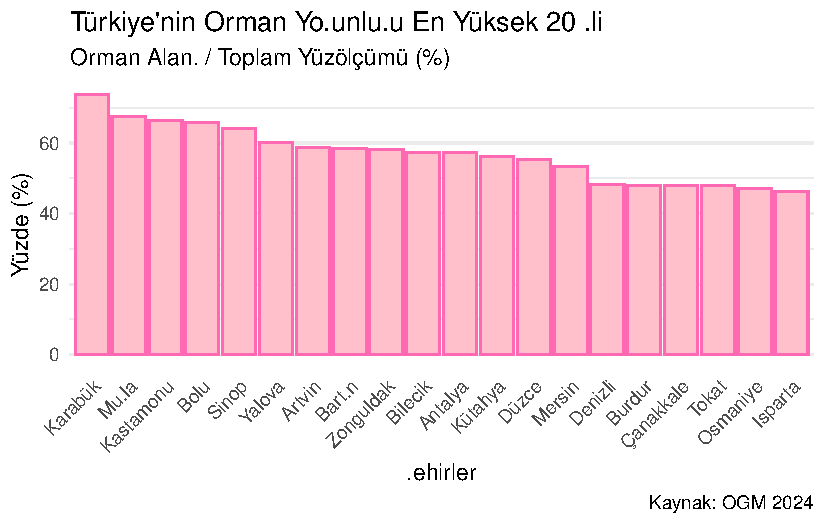
\includegraphics[keepaspectratio]{data_files/figure-pdf/unnamed-chunk-9-1.pdf}}

2)For the temporal part of our analysis, we focused on forest fire
trends and the total extent of burned areas over the last two decades.
Our primary expectation was to see the Mediterranean coast as the most
affected region, given its climate and high vegetation density. We
wanted to see if the data confirms this regional risk and how the
numbers have fluctuated over the years. To prepare this section, we
processed long-term statistics from OGM, ensuring the time-series data
was consistent and free of missing values. This allowed us to compare
our ``common knowledge'' about Mediterranean fire risks with the actual
historical records.

\section{FORESTS FIRES NUMBERS AND AREA ANALYSIS BY
CITIES}\label{forests-fires-numbers-and-area-analysis-by-cities}

\section{1.installing packages}\label{installing-packages}

\begin{Shaded}
\begin{Highlighting}[]
\FunctionTok{library}\NormalTok{(sf)}
\end{Highlighting}
\end{Shaded}

\begin{verbatim}
Linking to GEOS 3.13.0, GDAL 3.8.5, PROJ 9.5.1; sf_use_s2() is TRUE
\end{verbatim}

\begin{Shaded}
\begin{Highlighting}[]
\FunctionTok{library}\NormalTok{(tidyverse)}
\FunctionTok{library}\NormalTok{(readxl)}
\FunctionTok{library}\NormalTok{(scales) }
\end{Highlighting}
\end{Shaded}

\begin{verbatim}

Attaching package: 'scales'
\end{verbatim}

\begin{verbatim}
The following object is masked from 'package:purrr':

    discard
\end{verbatim}

\begin{verbatim}
The following object is masked from 'package:readr':

    col_factor
\end{verbatim}

\section{2. introducing the file
paths}\label{introducing-the-file-paths}

\begin{Shaded}
\begin{Highlighting}[]
\NormalTok{harita\_yolu }\OtherTok{\textless{}{-}} \StringTok{"/Users/zzunb/Downloads/tr{-}cities.json"}
\NormalTok{adet\_yolu }\OtherTok{\textless{}{-}} \StringTok{"/Users/zzunb/Downloads/illere\_gore\_yangin\_adet\_2004{-}2024.xlsx"}
\NormalTok{alan\_yolu }\OtherTok{\textless{}{-}} \StringTok{"/Users/zzunb/Downloads/illere\_gore\_yanan\_alan\_2004{-}2024.xlsx"}
\end{Highlighting}
\end{Shaded}

\section{3. reading data and type
conversion}\label{reading-data-and-type-conversion}

\begin{Shaded}
\begin{Highlighting}[]
\NormalTok{tr\_map }\OtherTok{\textless{}{-}} \FunctionTok{read\_sf}\NormalTok{(harita\_yolu)}
\NormalTok{df\_adet\_ham }\OtherTok{\textless{}{-}} \FunctionTok{read\_excel}\NormalTok{(adet\_yolu, }\AttributeTok{skip =} \DecValTok{3}\NormalTok{)}
\end{Highlighting}
\end{Shaded}

\begin{verbatim}
New names:
* `` -> `...1`
\end{verbatim}

\begin{Shaded}
\begin{Highlighting}[]
\FunctionTok{colnames}\NormalTok{(df\_adet\_ham)[}\DecValTok{1}\NormalTok{] }\OtherTok{\textless{}{-}} \StringTok{"Bolge"}
\NormalTok{df\_adet\_ham }\OtherTok{\textless{}{-}}\NormalTok{ df\_adet\_ham }\SpecialCharTok{\%\textgreater{}\%} 
  \FunctionTok{filter}\NormalTok{(}\SpecialCharTok{!}\FunctionTok{is.na}\NormalTok{(Bolge)) }\SpecialCharTok{\%\textgreater{}\%} 
  \FunctionTok{slice}\NormalTok{(}\DecValTok{1}\SpecialCharTok{:}\NormalTok{(}\FunctionTok{which}\NormalTok{(Bolge }\SpecialCharTok{==} \StringTok{"Zonguldak"}\NormalTok{))) }\SpecialCharTok{\%\textgreater{}\%}
  \FunctionTok{mutate}\NormalTok{(}\FunctionTok{across}\NormalTok{(}\SpecialCharTok{{-}}\NormalTok{Bolge, }\SpecialCharTok{\textasciitilde{}} \FunctionTok{suppressWarnings}\NormalTok{(}\FunctionTok{as.numeric}\NormalTok{(.))))}

\NormalTok{df\_alan\_ham }\OtherTok{\textless{}{-}} \FunctionTok{read\_excel}\NormalTok{(alan\_yolu, }\AttributeTok{skip =} \DecValTok{3}\NormalTok{)}
\end{Highlighting}
\end{Shaded}

\begin{verbatim}
New names:
* `` -> `...1`
\end{verbatim}

\begin{Shaded}
\begin{Highlighting}[]
\FunctionTok{colnames}\NormalTok{(df\_alan\_ham)[}\DecValTok{1}\NormalTok{] }\OtherTok{\textless{}{-}} \StringTok{"Bolge"}
\NormalTok{df\_alan\_ham }\OtherTok{\textless{}{-}}\NormalTok{ df\_alan\_ham }\SpecialCharTok{\%\textgreater{}\%} 
  \FunctionTok{filter}\NormalTok{(}\SpecialCharTok{!}\FunctionTok{is.na}\NormalTok{(Bolge)) }\SpecialCharTok{\%\textgreater{}\%} 
  \FunctionTok{slice}\NormalTok{(}\DecValTok{1}\SpecialCharTok{:}\NormalTok{(}\FunctionTok{which}\NormalTok{(Bolge }\SpecialCharTok{==} \StringTok{"Zonguldak"}\NormalTok{))) }\SpecialCharTok{\%\textgreater{}\%}
  \FunctionTok{mutate}\NormalTok{(}\FunctionTok{across}\NormalTok{(}\SpecialCharTok{{-}}\NormalTok{Bolge, }\SpecialCharTok{\textasciitilde{}} \FunctionTok{suppressWarnings}\NormalTok{(}\FunctionTok{as.numeric}\NormalTok{(.))))}
\end{Highlighting}
\end{Shaded}

\section{4. data cleaning calculating totals (AI
help)}\label{data-cleaning-calculating-totals-ai-help}

\begin{Shaded}
\begin{Highlighting}[]
\NormalTok{temizle\_ve\_topla }\OtherTok{\textless{}{-}} \ControlFlowTok{function}\NormalTok{(df) \{}
\NormalTok{  df\_sonuc }\OtherTok{\textless{}{-}}\NormalTok{ df }\SpecialCharTok{\%\textgreater{}\%} 
    \FunctionTok{filter}\NormalTok{(}\SpecialCharTok{!}\NormalTok{Bolge }\SpecialCharTok{\%in\%} \FunctionTok{c}\NormalTok{(}\StringTok{"Toplam{-}Total"}\NormalTok{, }\StringTok{"DKMPGM"}\NormalTok{)) }\SpecialCharTok{\%\textgreater{}\%}
    \FunctionTok{mutate}\NormalTok{(}\AttributeTok{Bolge =} \FunctionTok{recode}\NormalTok{(Bolge, }\StringTok{"K.Maraş"} \OtherTok{=} \StringTok{"Kahramanmaraş"}\NormalTok{, }\StringTok{"Afyon"} \OtherTok{=} \StringTok{"Afyonkarahisar"}\NormalTok{)) }\SpecialCharTok{\%\textgreater{}\%}
    \FunctionTok{rowwise}\NormalTok{() }\SpecialCharTok{\%\textgreater{}\%}
    \FunctionTok{mutate}\NormalTok{(}\AttributeTok{Toplam\_21\_Yil =} \FunctionTok{sum}\NormalTok{(}\FunctionTok{c\_across}\NormalTok{(}\FunctionTok{where}\NormalTok{(is.numeric)), }\AttributeTok{na.rm =} \ConstantTok{TRUE}\NormalTok{)) }\SpecialCharTok{\%\textgreater{}\%}
    \FunctionTok{ungroup}\NormalTok{()}
  
  \FunctionTok{return}\NormalTok{(df\_sonuc)}
\NormalTok{\}}

\NormalTok{df\_adet }\OtherTok{\textless{}{-}} \FunctionTok{temizle\_ve\_topla}\NormalTok{(df\_adet\_ham) }\SpecialCharTok{\%\textgreater{}\%} \FunctionTok{arrange}\NormalTok{(}\FunctionTok{desc}\NormalTok{(Toplam\_21\_Yil))}
\NormalTok{df\_alan }\OtherTok{\textless{}{-}} \FunctionTok{temizle\_ve\_topla}\NormalTok{(df\_alan\_ham) }\SpecialCharTok{\%\textgreater{}\%} \FunctionTok{arrange}\NormalTok{(}\FunctionTok{desc}\NormalTok{(Toplam\_21\_Yil))}

\FunctionTok{print}\NormalTok{(}\StringTok{"{-}{-}{-} YANGIN ADETLERİ {-}{-}{-}"}\NormalTok{)}
\end{Highlighting}
\end{Shaded}

\begin{verbatim}
[1] "--- YANGIN ADETLERİ ---"
\end{verbatim}

\begin{Shaded}
\begin{Highlighting}[]
\NormalTok{knitr}\SpecialCharTok{::}\FunctionTok{kable}\NormalTok{(df\_adet)}
\end{Highlighting}
\end{Shaded}

{\def\LTcaptype{none} % do not increment counter
\begin{longtable}[]{@{}
  >{\raggedright\arraybackslash}p{(\linewidth - 44\tabcolsep) * \real{0.1053}}
  >{\raggedleft\arraybackslash}p{(\linewidth - 44\tabcolsep) * \real{0.0376}}
  >{\raggedleft\arraybackslash}p{(\linewidth - 44\tabcolsep) * \real{0.0376}}
  >{\raggedleft\arraybackslash}p{(\linewidth - 44\tabcolsep) * \real{0.0376}}
  >{\raggedleft\arraybackslash}p{(\linewidth - 44\tabcolsep) * \real{0.0376}}
  >{\raggedleft\arraybackslash}p{(\linewidth - 44\tabcolsep) * \real{0.0376}}
  >{\raggedleft\arraybackslash}p{(\linewidth - 44\tabcolsep) * \real{0.0376}}
  >{\raggedleft\arraybackslash}p{(\linewidth - 44\tabcolsep) * \real{0.0376}}
  >{\raggedleft\arraybackslash}p{(\linewidth - 44\tabcolsep) * \real{0.0376}}
  >{\raggedleft\arraybackslash}p{(\linewidth - 44\tabcolsep) * \real{0.0376}}
  >{\raggedleft\arraybackslash}p{(\linewidth - 44\tabcolsep) * \real{0.0376}}
  >{\raggedleft\arraybackslash}p{(\linewidth - 44\tabcolsep) * \real{0.0376}}
  >{\raggedleft\arraybackslash}p{(\linewidth - 44\tabcolsep) * \real{0.0376}}
  >{\raggedleft\arraybackslash}p{(\linewidth - 44\tabcolsep) * \real{0.0376}}
  >{\raggedleft\arraybackslash}p{(\linewidth - 44\tabcolsep) * \real{0.0376}}
  >{\raggedleft\arraybackslash}p{(\linewidth - 44\tabcolsep) * \real{0.0376}}
  >{\raggedleft\arraybackslash}p{(\linewidth - 44\tabcolsep) * \real{0.0376}}
  >{\raggedleft\arraybackslash}p{(\linewidth - 44\tabcolsep) * \real{0.0376}}
  >{\raggedleft\arraybackslash}p{(\linewidth - 44\tabcolsep) * \real{0.0376}}
  >{\raggedleft\arraybackslash}p{(\linewidth - 44\tabcolsep) * \real{0.0376}}
  >{\raggedleft\arraybackslash}p{(\linewidth - 44\tabcolsep) * \real{0.0376}}
  >{\raggedleft\arraybackslash}p{(\linewidth - 44\tabcolsep) * \real{0.0376}}
  >{\raggedleft\arraybackslash}p{(\linewidth - 44\tabcolsep) * \real{0.1053}}@{}}
\toprule\noalign{}
\begin{minipage}[b]{\linewidth}\raggedright
Bolge
\end{minipage} & \begin{minipage}[b]{\linewidth}\raggedleft
2004
\end{minipage} & \begin{minipage}[b]{\linewidth}\raggedleft
2005
\end{minipage} & \begin{minipage}[b]{\linewidth}\raggedleft
2006
\end{minipage} & \begin{minipage}[b]{\linewidth}\raggedleft
2007
\end{minipage} & \begin{minipage}[b]{\linewidth}\raggedleft
2008
\end{minipage} & \begin{minipage}[b]{\linewidth}\raggedleft
2009
\end{minipage} & \begin{minipage}[b]{\linewidth}\raggedleft
2010
\end{minipage} & \begin{minipage}[b]{\linewidth}\raggedleft
2011
\end{minipage} & \begin{minipage}[b]{\linewidth}\raggedleft
2012
\end{minipage} & \begin{minipage}[b]{\linewidth}\raggedleft
2013
\end{minipage} & \begin{minipage}[b]{\linewidth}\raggedleft
2014
\end{minipage} & \begin{minipage}[b]{\linewidth}\raggedleft
2015
\end{minipage} & \begin{minipage}[b]{\linewidth}\raggedleft
2016
\end{minipage} & \begin{minipage}[b]{\linewidth}\raggedleft
2017
\end{minipage} & \begin{minipage}[b]{\linewidth}\raggedleft
2018
\end{minipage} & \begin{minipage}[b]{\linewidth}\raggedleft
2019
\end{minipage} & \begin{minipage}[b]{\linewidth}\raggedleft
2020
\end{minipage} & \begin{minipage}[b]{\linewidth}\raggedleft
2021
\end{minipage} & \begin{minipage}[b]{\linewidth}\raggedleft
2022
\end{minipage} & \begin{minipage}[b]{\linewidth}\raggedleft
2023
\end{minipage} & \begin{minipage}[b]{\linewidth}\raggedleft
2024
\end{minipage} & \begin{minipage}[b]{\linewidth}\raggedleft
Toplam\_21\_Yil
\end{minipage} \\
\midrule\noalign{}
\endhead
\bottomrule\noalign{}
\endlastfoot
Muğla & 224 & 255 & 326 & 415 & 348 & 252 & 309 & 267 & 383 & 395 & 320
& 254 & 373 & 233 & 355 & 302 & 329 & 364 & 273 & 317 & 377 & 6671 \\
İzmir & 185 & 139 & 179 & 256 & 151 & 183 & 216 & 197 & 269 & 344 & 284
& 265 & 377 & 233 & 264 & 240 & 285 & 262 & 293 & 314 & 397 & 5333 \\
Antalya & 241 & 278 & 240 & 265 & 212 & 144 & 125 & 152 & 214 & 321 &
169 & 189 & 281 & 273 & 244 & 199 & 260 & 278 & 179 & 162 & 248 &
4674 \\
İstanbul & 68 & 58 & 151 & 186 & 136 & 115 & 42 & 172 & 228 & 271 & 108
& 153 & 254 & 173 & 82 & 204 & 197 & 81 & 92 & 145 & 144 & 3060 \\
Kahramanmaraş & 63 & 68 & 71 & 100 & 64 & 79 & 119 & 78 & 132 & 262 &
155 & 170 & 232 & 183 & 169 & 160 & 264 & 200 & 84 & 142 & 232 & 3027 \\
Adana & 89 & 64 & 105 & 123 & 107 & 83 & 84 & 88 & 101 & 173 & 81 & 176
& 183 & 151 & 124 & 174 & 186 & 190 & 108 & 132 & 132 & 2654 \\
Amasya & 68 & 52 & 116 & 165 & 63 & 74 & 104 & 93 & 95 & 144 & 84 & 60 &
121 & 79 & 86 & 81 & 158 & 81 & 47 & 77 & 182 & 2030 \\
Mersin & 59 & 48 & 50 & 128 & 93 & 60 & 90 & 98 & 75 & 155 & 91 & 80 &
107 & 54 & 71 & 90 & 87 & 89 & 99 & 82 & 107 & 1813 \\
Kastamonu & 46 & 53 & 97 & 169 & 67 & 39 & 48 & 63 & 120 & 146 & 88 & 57
& 82 & 108 & 66 & 98 & 211 & 78 & 37 & 43 & 80 & 1796 \\
Şanlıurfa & NA & NA & NA & NA & NA & NA & NA & 21 & 23 & 101 & 66 & 89 &
150 & 80 & 125 & 121 & 242 & 163 & 102 & 210 & 274 & 1767 \\
Balıkesir & 104 & 76 & 105 & 122 & 80 & 90 & 57 & 79 & 73 & 96 & 72 & 68
& 73 & 56 & 60 & 71 & 80 & 87 & 91 & 68 & 105 & 1713 \\
Denizli & 129 & 115 & 128 & 154 & 90 & 79 & 72 & 76 & 68 & 146 & 47 & 41
& 84 & 45 & 33 & 24 & 39 & 67 & 50 & 37 & 120 & 1644 \\
Bursa & 66 & 34 & 82 & 94 & 97 & 105 & 53 & 72 & 81 & 118 & 64 & 43 & 78
& 63 & 40 & 84 & 69 & 61 & 80 & 77 & 120 & 1581 \\
Ankara & 59 & 47 & 76 & 95 & 38 & 84 & 57 & 73 & 113 & 233 & 46 & 43 &
125 & 98 & 46 & 55 & 67 & 46 & 33 & 53 & 75 & 1562 \\
Elazığ & 14 & 16 & 27 & 56 & 77 & 45 & 47 & 14 & 4 & 72 & 79 & 84 & 80 &
42 & 47 & 157 & 149 & 142 & 53 & 82 & 170 & 1457 \\
Isparta & 49 & 28 & 47 & 53 & 69 & 76 & 78 & 56 & 105 & 120 & 70 & 74 &
54 & 54 & 48 & 67 & 71 & 50 & 39 & 46 & 77 & 1331 \\
Sakarya & 36 & 27 & 57 & 80 & 98 & 74 & 54 & 58 & 56 & 78 & 33 & 46 & 61
& 50 & 31 & 66 & 135 & 43 & 59 & 60 & 73 & 1275 \\
Zonguldak & 59 & 63 & 137 & 108 & 111 & 30 & 44 & 57 & 57 & 85 & 46 & 47
& 48 & 66 & 25 & 20 & 62 & 32 & 17 & 37 & 64 & 1215 \\
Kütahya & 57 & 26 & 46 & 63 & 48 & 55 & 34 & 41 & 54 & 90 & 55 & 33 & 68
& 48 & 52 & 38 & 58 & 42 & 57 & 32 & 112 & 1109 \\
Çanakkale & NA & NA & NA & NA & NA & NA & NA & NA & NA & NA & NA & NA &
63 & 44 & 56 & 92 & 123 & 84 & 131 & 145 & 144 & 882 \\
Giresun & 13 & 8 & 11 & 19 & 27 & 9 & 60 & 16 & 30 & 40 & 46 & 43 & 38 &
36 & 18 & 64 & 71 & 95 & 25 & 43 & 96 & 808 \\
Bolu & 21 & 17 & 57 & 61 & 45 & 18 & 30 & 32 & 40 & 57 & 26 & 24 & 44 &
30 & 25 & 54 & 58 & 33 & 20 & 40 & 56 & 788 \\
Eskişehir & 46 & 16 & 43 & 59 & 42 & 51 & 44 & 32 & 38 & 79 & 21 & 12 &
55 & 33 & 25 & 35 & 23 & 17 & 19 & 31 & 54 & 775 \\
Konya & 35 & 24 & 42 & 37 & 30 & 36 & 51 & 32 & 50 & 91 & 31 & 29 & 47 &
13 & 20 & 30 & 34 & 23 & 4 & 13 & 43 & 715 \\
Trabzon & 9 & 11 & 3 & 5 & 26 & 9 & 25 & 21 & 6 & 41 & 29 & 22 & 27 & 38
& 18 & 73 & 61 & 68 & 24 & 46 & 71 & 633 \\
Kayseri & NA & NA & NA & NA & NA & NA & NA & 54 & 16 & 69 & 27 & 26 & 74
& 38 & 23 & 18 & 28 & 21 & 18 & 23 & 74 & 509 \\
Erzurum & 18 & 2 & 26 & 8 & 8 & 2 & 1 & 7 & 16 & 21 & 5 & 17 & 9 & 79 &
11 & 48 & 33 & 37 & 24 & 18 & 7 & 397 \\
Artvin & 4 & 5 & 5 & 8 & 8 & NA & 17 & 5 & 3 & 7 & 6 & 5 & NA & 11 & 3 &
23 & 19 & 23 & 12 & 4 & 18 & 186 \\
Hatay & NA & NA & NA & NA & NA & NA & NA & NA & NA & NA & NA & NA & NA &
NA & NA & NA & NA & NA & 56 & 49 & 53 & 158 \\
Sinop & NA & NA & NA & NA & NA & NA & NA & NA & NA & NA & NA & NA & NA &
NA & NA & NA & NA & NA & 6 & 27 & 40 & 73 \\
\end{longtable}
}

\begin{Shaded}
\begin{Highlighting}[]
\FunctionTok{print}\NormalTok{(}\StringTok{"{-}{-}{-} YANAN ALANLAR {-}{-}{-}"}\NormalTok{)}
\end{Highlighting}
\end{Shaded}

\begin{verbatim}
[1] "--- YANAN ALANLAR ---"
\end{verbatim}

\begin{Shaded}
\begin{Highlighting}[]
\NormalTok{knitr}\SpecialCharTok{::}\FunctionTok{kable}\NormalTok{(df\_alan)}
\end{Highlighting}
\end{Shaded}

{\def\LTcaptype{none} % do not increment counter
\begin{longtable}[]{@{}
  >{\raggedright\arraybackslash}p{(\linewidth - 44\tabcolsep) * \real{0.0778}}
  >{\raggedleft\arraybackslash}p{(\linewidth - 44\tabcolsep) * \real{0.0278}}
  >{\raggedleft\arraybackslash}p{(\linewidth - 44\tabcolsep) * \real{0.0444}}
  >{\raggedleft\arraybackslash}p{(\linewidth - 44\tabcolsep) * \real{0.0389}}
  >{\raggedleft\arraybackslash}p{(\linewidth - 44\tabcolsep) * \real{0.0556}}
  >{\raggedleft\arraybackslash}p{(\linewidth - 44\tabcolsep) * \real{0.0333}}
  >{\raggedleft\arraybackslash}p{(\linewidth - 44\tabcolsep) * \real{0.0500}}
  >{\raggedleft\arraybackslash}p{(\linewidth - 44\tabcolsep) * \real{0.0278}}
  >{\raggedleft\arraybackslash}p{(\linewidth - 44\tabcolsep) * \real{0.0444}}
  >{\raggedleft\arraybackslash}p{(\linewidth - 44\tabcolsep) * \real{0.0500}}
  >{\raggedleft\arraybackslash}p{(\linewidth - 44\tabcolsep) * \real{0.0500}}
  >{\raggedleft\arraybackslash}p{(\linewidth - 44\tabcolsep) * \real{0.0389}}
  >{\raggedleft\arraybackslash}p{(\linewidth - 44\tabcolsep) * \real{0.0278}}
  >{\raggedleft\arraybackslash}p{(\linewidth - 44\tabcolsep) * \real{0.0278}}
  >{\raggedleft\arraybackslash}p{(\linewidth - 44\tabcolsep) * \real{0.0278}}
  >{\raggedleft\arraybackslash}p{(\linewidth - 44\tabcolsep) * \real{0.0278}}
  >{\raggedleft\arraybackslash}p{(\linewidth - 44\tabcolsep) * \real{0.0556}}
  >{\raggedleft\arraybackslash}p{(\linewidth - 44\tabcolsep) * \real{0.0556}}
  >{\raggedleft\arraybackslash}p{(\linewidth - 44\tabcolsep) * \real{0.0611}}
  >{\raggedleft\arraybackslash}p{(\linewidth - 44\tabcolsep) * \real{0.0444}}
  >{\raggedleft\arraybackslash}p{(\linewidth - 44\tabcolsep) * \real{0.0278}}
  >{\raggedleft\arraybackslash}p{(\linewidth - 44\tabcolsep) * \real{0.0278}}
  >{\raggedleft\arraybackslash}p{(\linewidth - 44\tabcolsep) * \real{0.0778}}@{}}
\toprule\noalign{}
\begin{minipage}[b]{\linewidth}\raggedright
Bolge
\end{minipage} & \begin{minipage}[b]{\linewidth}\raggedleft
2004
\end{minipage} & \begin{minipage}[b]{\linewidth}\raggedleft
2005
\end{minipage} & \begin{minipage}[b]{\linewidth}\raggedleft
2006
\end{minipage} & \begin{minipage}[b]{\linewidth}\raggedleft
2007
\end{minipage} & \begin{minipage}[b]{\linewidth}\raggedleft
2008
\end{minipage} & \begin{minipage}[b]{\linewidth}\raggedleft
2009
\end{minipage} & \begin{minipage}[b]{\linewidth}\raggedleft
2010
\end{minipage} & \begin{minipage}[b]{\linewidth}\raggedleft
2011
\end{minipage} & \begin{minipage}[b]{\linewidth}\raggedleft
2012
\end{minipage} & \begin{minipage}[b]{\linewidth}\raggedleft
2013
\end{minipage} & \begin{minipage}[b]{\linewidth}\raggedleft
2014
\end{minipage} & \begin{minipage}[b]{\linewidth}\raggedleft
2015
\end{minipage} & \begin{minipage}[b]{\linewidth}\raggedleft
2016
\end{minipage} & \begin{minipage}[b]{\linewidth}\raggedleft
2017
\end{minipage} & \begin{minipage}[b]{\linewidth}\raggedleft
2018
\end{minipage} & \begin{minipage}[b]{\linewidth}\raggedleft
2019
\end{minipage} & \begin{minipage}[b]{\linewidth}\raggedleft
2020
\end{minipage} & \begin{minipage}[b]{\linewidth}\raggedleft
2021
\end{minipage} & \begin{minipage}[b]{\linewidth}\raggedleft
2022
\end{minipage} & \begin{minipage}[b]{\linewidth}\raggedleft
2023
\end{minipage} & \begin{minipage}[b]{\linewidth}\raggedleft
2024
\end{minipage} & \begin{minipage}[b]{\linewidth}\raggedleft
Toplam\_21\_Yil
\end{minipage} \\
\midrule\noalign{}
\endhead
\bottomrule\noalign{}
\endlastfoot
Antalya & 509 & 404.490 & 514.7 & 2093.2000 & 17026 & 468.750 & 503 &
91.885 & 652.677 & 1312.100 & 234.00 & 197 & 2159 & 2750 & 594 &
234.8600 & 399.5840 & 60357.9197 & 200.69 & 386 & 333 & 91421.8557 \\
Muğla & 258 & 944.600 & 3416.1 & 1531.4000 & 665 & 259.700 & 160 &
165.400 & 241.851 & 971.536 & 724.00 & 184 & 481 & 442 & 232 & 960.3510
& 815.1920 & 43100.5089 & 5344.88 & 402 & 3466 & 64765.5189 \\
İzmir & 976 & 438.100 & 579.3 & 963.0000 & 1790 & 1603.114 & 502 &
732.745 & 474.211 & 862.244 & 270.04 & 153 & 1041 & 2022 & 392 &
4903.9855 & 4110.2168 & 824.7473 & 1300.26 & 2734 & 9176 & 35847.9636 \\
Mersin & 24 & 13.700 & 29.3 & 1053.1510 & 5080 & 79.932 & 105 & 113.670
& 505.115 & 509.170 & 79.00 & 282 & 198 & 928 & 70 & 360.7900 & 509.1530
& 9661.2010 & 2118.13 & 898 & 69 & 22686.3120 \\
Kahramanmaraş & 119 & 93.300 & 44.7 & 948.6800 & 710 & 77.610 & 162 &
204.370 & 3669.100 & 1579.470 & 159.60 & 184 & 315 & 249 & 1489 &
626.3290 & 5408.6886 & 899.7864 & 70.56 & 522 & 992 & 18524.1940 \\
Adana & 397 & 94.000 & 443.2 & 704.4300 & 415 & 183.180 & 237 & 222.450
& 916.310 & 874.920 & 144.78 & 402 & 177 & 162 & 163 & 159.0787 &
2775.5371 & 7698.6000 & 486.49 & 346 & 123 & 17124.9758 \\
Balıkesir & 964 & 267.000 & 302.0 & 543.0000 & 1974 & 328.000 & 64 &
420.836 & 658.247 & 2350.233 & 33.49 & 39 & 601 & 168 & 24 & 74.7840 &
104.2300 & 63.7000 & 181.23 & 97 & 261 & 9518.7500 \\
Şanlıurfa & NA & NA & NA & NA & NA & NA & NA & 44.570 & 89.150 & 387.090
& 302.00 & 536 & 1302 & 1133 & 1385 & 1033.1800 & 423.3660 & 390.0500 &
387.16 & 573 & 1042 & 9027.5660 \\
Çanakkale & NA & NA & NA & NA & NA & NA & NA & NA & NA & NA & NA & NA &
505 & 320 & 130 & 290.4300 & 930.0130 & 106.7205 & 602.80 & 5357 & 481 &
8722.9635 \\
Elazığ & 217 & 114.500 & 104.4 & 338.0000 & 859 & 210.100 & 235 & 73.300
& 20.200 & 53.100 & 63.05 & 71 & 41 & 26 & 81 & 652.3700 & 210.2989 &
2657.1450 & 167.31 & 485 & 731 & 7409.7739 \\
Denizli & 181 & 46.970 & 60.9 & 368.9200 & 71 & 87.600 & 91 & 116.311 &
234.960 & 122.082 & 79.82 & 34 & 117 & 444 & 84 & 13.4200 & 541.8300 &
1074.2419 & 287.41 & 55 & 2653 & 6764.4649 \\
Bolu & 19 & 18.110 & 283.6 & 79.9819 & 29 & 12.265 & 85 & 83.273 &
64.513 & 77.157 & 14.01 & 51 & 30 & 279 & 22 & 42.1300 & 203.6640 &
27.7471 & 15.11 & 415 & 3619 & 5470.5610 \\
Bursa & 105 & 10.710 & 159.3 & 386.2500 & 54 & 451.967 & 108 & 120.940 &
342.949 & 532.400 & 39.56 & 263 & 139 & 254 & 62 & 304.4000 & 97.3525 &
35.1053 & 280.59 & 395 & 734 & 4875.5238 \\
Kütahya & 251 & 8.000 & 574.4 & 581.3000 & 15 & 25.480 & 11 & 14.330 &
182.605 & 71.580 & 52.00 & 6 & 285 & 860 & 45 & 112.1700 & 117.9600 &
23.6200 & 275.93 & 230 & 121 & 3863.3750 \\
Kastamonu & 43 & 53.000 & 166.0 & 311.0000 & 83 & 26.000 & 48 & 39.744 &
204.510 & 76.827 & 45.52 & 30 & 41 & 104 & 299 & 110.3400 & 1958.9790 &
61.7000 & 5.14 & 16 & 74 & 3796.7600 \\
Amasya & 108 & 31.800 & 93.4 & 413.4120 & 46 & 84.827 & 306 & 158.070 &
139.140 & 279.520 & 200.57 & 119 & 390 & 137 & 52 & 150.9900 & 562.4700
& 80.8000 & 59.15 & 89 & 247 & 3748.1490 \\
Isparta & 48 & 10.345 & 48.8 & 54.6130 & 61 & 38.296 & 130 & 127.180 &
297.480 & 97.090 & 60.62 & 54 & 32 & 104 & 41 & 139.6452 & 49.2900 &
2042.5653 & 21.23 & 81 & 42 & 3580.1545 \\
Ankara & 173 & 41.970 & 313.5 & 80.4300 & 63 & 65.065 & 43 & 165.302 &
158.488 & 176.542 & 35.93 & 15 & 414 & 92 & 80 & 69.6000 & 781.1300 &
25.9140 & 4.94 & 257 & 253 & 3308.8110 \\
İstanbul & 145 & 31.910 & 66.5 & 262.9520 & 96 & 89.974 & 8 & 67.039 &
107.331 & 76.603 & 18.00 & 41 & 92 & 39 & 26 & 54.4430 & 316.2498 &
42.9629 & 73.39 & 292 & 583 & 2529.3547 \\
Trabzon & 73 & 57.500 & 10.1 & 40.0000 & 324 & 45.720 & 61 & 72.993 &
38.500 & 166.410 & 268.00 & 141 & 60 & 167 & 32 & 443.8000 & 100.1060 &
194.6127 & 25.44 & 72 & 87 & 2480.1817 \\
Zonguldak & 36 & 62.793 & 100.7 & 373.4550 & 56 & 13.505 & 71 & 90.619 &
1013.135 & 56.674 & 19.00 & 111 & 28 & 74 & 14 & 10.5900 & 85.4500 &
62.4063 & 2.99 & 19 & 145 & 2445.3173 \\
Sakarya & 77 & 24.830 & 170.0 & 320.5100 & 192 & 358.060 & 87 & 106.463
& 99.134 & 116.520 & 28.00 & 34 & 46 & 82 & 11 & 56.0700 & 90.0170 &
15.6938 & 32.57 & 48 & 60 & 2054.8678 \\
Erzurum & 50 & 2.400 & 64.8 & 27.9000 & 14 & NA & NA & 40.000 & 65.520 &
55.400 & 8.80 & 83 & 69 & 901 & 33 & 209.5000 & 56.9200 & 61.9900 &
132.67 & 21 & 2 & 1898.9000 \\
Eskişehir & 38 & 11.450 & 65.7 & 107.0300 & 24 & 70.400 & 46 & 54.440 &
104.600 & 155.320 & 21.80 & 5 & 225 & 75 & 14 & 75.0000 & 68.0550 &
11.8200 & 35.28 & 394 & 144 & 1745.8950 \\
Kayseri & NA & NA & NA & NA & NA & NA & NA & 160.850 & 50.660 & 203.020
& 69.00 & 41 & 214 & 104 & 111 & 35.2600 & 80.6900 & 17.8700 & 15.04 &
98 & 228 & 1428.3900 \\
Konya & 39 & 12.130 & 132.4 & 42.1700 & 17 & 87.550 & 106 & 78.430 &
84.990 & 182.493 & 49.00 & 64 & 84 & 11 & 106 & 63.7830 & 71.5400 &
17.4905 & 0.63 & 32 & 64 & 1345.6065 \\
Giresun & 22 & 17.900 & 10.2 & 33.4800 & 51 & 10.850 & 106 & 26.790 &
32.313 & 91.490 & 89.12 & 74 & 70 & 61 & 51 & 128.4400 & 84.7111 &
146.8548 & 54.56 & 53 & 107 & 1321.7089 \\
Hatay & NA & NA & NA & NA & NA & NA & NA & NA & NA & NA & NA & NA & NA &
NA & NA & NA & NA & NA & 121.64 & 732 & 290 & 1143.6400 \\
Artvin & 4 & 9.310 & 7.3 & 6.3600 & 34 & NA & 42 & 20.000 & 6.948 &
19.500 & 8.63 & 5 & NA & 5 & 1 & 16.6966 & 18.2507 & 24.2700 & 18.73 & 3
& 3 & 252.9953 \\
Sinop & NA & NA & NA & NA & NA & NA & NA & NA & NA & NA & NA & NA & NA &
NA & NA & NA & NA & NA & 2.18 & 12 & 66 & 80.1800 \\
\end{longtable}
}

3)In the final part of our data preparation, we focused on the specific
causes behind forest fires in recent years. Our main expectation was to
find that negligence and human error---such as stubble burning or
unattended campfires---are the leading drivers of these incidents. We
wanted to analyze the categorical breakdown of these causes to see how
much of the damage could have been prevented through better awareness.
To make this data ready for analysis, we categorized the OGM statistics
for the 2022-2024 period, ensuring the labels were clear and consistent.
This step was crucial for us to move beyond just looking at the
``where'' and ``when'' of fires, and start understanding the ``why.''

\section{FOREST FIRES CAUSING MAIN
REASONS}\label{forest-fires-causing-main-reasons}

\section{1. loading packages}\label{loading-packages}

\begin{Shaded}
\begin{Highlighting}[]
\FunctionTok{library}\NormalTok{(sf)}
\FunctionTok{library}\NormalTok{(tidyverse)}
\FunctionTok{library}\NormalTok{(readxl)}
\end{Highlighting}
\end{Shaded}

\section{2. defining file paths}\label{defining-file-paths}

\begin{Shaded}
\begin{Highlighting}[]
\NormalTok{harita\_yolu }\OtherTok{\textless{}{-}} \StringTok{"/Users/zzunb/Downloads/tr{-}cities.json"}
\NormalTok{excel\_yolu }\OtherTok{\textless{}{-}} \StringTok{"/Users/zzunb/Downloads/2022{-}2024\_sebep\_adet\_toplam.xlsx"}
\end{Highlighting}
\end{Shaded}

\section{3. reading the data}\label{reading-the-data}

\begin{Shaded}
\begin{Highlighting}[]
\NormalTok{tr\_map }\OtherTok{\textless{}{-}} \FunctionTok{read\_sf}\NormalTok{(harita\_yolu)}

\NormalTok{yangin\_verisi }\OtherTok{\textless{}{-}} \FunctionTok{read\_excel}\NormalTok{(excel\_yolu, }\AttributeTok{skip =} \DecValTok{5}\NormalTok{, }\AttributeTok{n\_max =} \DecValTok{31}\NormalTok{, }\AttributeTok{col\_names =} \ConstantTok{FALSE}\NormalTok{) }\SpecialCharTok{\%\textgreater{}\%}
  \FunctionTok{select}\NormalTok{(}
    \AttributeTok{Bolge =} \DecValTok{1}\NormalTok{,}
    \AttributeTok{Aniz =} \DecValTok{2}\NormalTok{, }\AttributeTok{Coplu =} \DecValTok{3}\NormalTok{, }\AttributeTok{Avcilik =} \DecValTok{4}\NormalTok{, }\AttributeTok{CobanAtesi =} \DecValTok{5}\NormalTok{, }\AttributeTok{Sigara =} \DecValTok{6}\NormalTok{, }\AttributeTok{Piknik =} \DecValTok{7}\NormalTok{, }\AttributeTok{Diger\_Ihmal =} \DecValTok{8}\NormalTok{,}
    \AttributeTok{Teror =} \DecValTok{10}\NormalTok{, }\AttributeTok{Kundaklama =} \DecValTok{11}\NormalTok{, }\AttributeTok{Acma =} \DecValTok{12}\NormalTok{, }\AttributeTok{Diger\_Kasit =} \DecValTok{13}\NormalTok{,}
    \AttributeTok{Enerji =} \DecValTok{15}\NormalTok{, }\AttributeTok{Trafik =} \DecValTok{16}\NormalTok{, }\AttributeTok{Diger\_Kaza =} \DecValTok{17}\NormalTok{,}
    \AttributeTok{Bilinmeyen =} \DecValTok{19}\NormalTok{, }\AttributeTok{Dogal =} \DecValTok{20}
\NormalTok{  ) }\SpecialCharTok{\%\textgreater{}\%}
  \FunctionTok{mutate}\NormalTok{(}\FunctionTok{across}\NormalTok{(}\SpecialCharTok{{-}}\NormalTok{Bolge, }\SpecialCharTok{\textasciitilde{}}\FunctionTok{as.numeric}\NormalTok{(}\FunctionTok{ifelse}\NormalTok{(. }\SpecialCharTok{==} \StringTok{"{-}"}\NormalTok{, }\StringTok{"0"}\NormalTok{, .)))) }\SpecialCharTok{\%\textgreater{}\%}
  \FunctionTok{filter}\NormalTok{(}\SpecialCharTok{!}\NormalTok{Bolge }\SpecialCharTok{\%in\%} \FunctionTok{c}\NormalTok{(}\StringTok{"DKMPGM"}\NormalTok{, }\StringTok{"Toplam{-}Total"}\NormalTok{))}
\end{Highlighting}
\end{Shaded}

\begin{verbatim}
New names:
* `` -> `...1`
* `` -> `...2`
* `` -> `...3`
* `` -> `...4`
* `` -> `...5`
* `` -> `...6`
* `` -> `...7`
* `` -> `...8`
* `` -> `...9`
* `` -> `...10`
* `` -> `...11`
* `` -> `...12`
* `` -> `...13`
* `` -> `...14`
* `` -> `...15`
* `` -> `...16`
* `` -> `...17`
* `` -> `...18`
* `` -> `...19`
* `` -> `...20`
* `` -> `...21`
\end{verbatim}

\begin{Shaded}
\begin{Highlighting}[]
\NormalTok{yangin\_verisi }\OtherTok{\textless{}{-}}\NormalTok{ yangin\_verisi }\SpecialCharTok{\%\textgreater{}\%}
  \FunctionTok{mutate}\NormalTok{(}\AttributeTok{Bolge =} \FunctionTok{recode}\NormalTok{(Bolge, }
                        \StringTok{"K.MaraE"} \OtherTok{=} \StringTok{"KahramanmaraE"}\NormalTok{,}
                        \StringTok{"Afyon"} \OtherTok{=} \StringTok{"Afyonkarahisar"}\NormalTok{))}
\NormalTok{knitr}\SpecialCharTok{::}\FunctionTok{kable}\NormalTok{(yangin\_verisi)}
\end{Highlighting}
\end{Shaded}

{\def\LTcaptype{none} % do not increment counter
\begin{longtable}[]{@{}
  >{\raggedright\arraybackslash}p{(\linewidth - 32\tabcolsep) * \real{0.0704}}
  >{\raggedleft\arraybackslash}p{(\linewidth - 32\tabcolsep) * \real{0.0352}}
  >{\raggedleft\arraybackslash}p{(\linewidth - 32\tabcolsep) * \real{0.0423}}
  >{\raggedleft\arraybackslash}p{(\linewidth - 32\tabcolsep) * \real{0.0563}}
  >{\raggedleft\arraybackslash}p{(\linewidth - 32\tabcolsep) * \real{0.0775}}
  >{\raggedleft\arraybackslash}p{(\linewidth - 32\tabcolsep) * \real{0.0493}}
  >{\raggedleft\arraybackslash}p{(\linewidth - 32\tabcolsep) * \real{0.0493}}
  >{\raggedleft\arraybackslash}p{(\linewidth - 32\tabcolsep) * \real{0.0845}}
  >{\raggedleft\arraybackslash}p{(\linewidth - 32\tabcolsep) * \real{0.0423}}
  >{\raggedleft\arraybackslash}p{(\linewidth - 32\tabcolsep) * \real{0.0775}}
  >{\raggedleft\arraybackslash}p{(\linewidth - 32\tabcolsep) * \real{0.0352}}
  >{\raggedleft\arraybackslash}p{(\linewidth - 32\tabcolsep) * \real{0.0845}}
  >{\raggedleft\arraybackslash}p{(\linewidth - 32\tabcolsep) * \real{0.0493}}
  >{\raggedleft\arraybackslash}p{(\linewidth - 32\tabcolsep) * \real{0.0493}}
  >{\raggedleft\arraybackslash}p{(\linewidth - 32\tabcolsep) * \real{0.0775}}
  >{\raggedleft\arraybackslash}p{(\linewidth - 32\tabcolsep) * \real{0.0775}}
  >{\raggedleft\arraybackslash}p{(\linewidth - 32\tabcolsep) * \real{0.0423}}@{}}
\toprule\noalign{}
\begin{minipage}[b]{\linewidth}\raggedright
Bolge
\end{minipage} & \begin{minipage}[b]{\linewidth}\raggedleft
Aniz
\end{minipage} & \begin{minipage}[b]{\linewidth}\raggedleft
Coplu
\end{minipage} & \begin{minipage}[b]{\linewidth}\raggedleft
Avcilik
\end{minipage} & \begin{minipage}[b]{\linewidth}\raggedleft
CobanAtesi
\end{minipage} & \begin{minipage}[b]{\linewidth}\raggedleft
Sigara
\end{minipage} & \begin{minipage}[b]{\linewidth}\raggedleft
Piknik
\end{minipage} & \begin{minipage}[b]{\linewidth}\raggedleft
Diger\_Ihmal
\end{minipage} & \begin{minipage}[b]{\linewidth}\raggedleft
Teror
\end{minipage} & \begin{minipage}[b]{\linewidth}\raggedleft
Kundaklama
\end{minipage} & \begin{minipage}[b]{\linewidth}\raggedleft
Acma
\end{minipage} & \begin{minipage}[b]{\linewidth}\raggedleft
Diger\_Kasit
\end{minipage} & \begin{minipage}[b]{\linewidth}\raggedleft
Enerji
\end{minipage} & \begin{minipage}[b]{\linewidth}\raggedleft
Trafik
\end{minipage} & \begin{minipage}[b]{\linewidth}\raggedleft
Diger\_Kaza
\end{minipage} & \begin{minipage}[b]{\linewidth}\raggedleft
Bilinmeyen
\end{minipage} & \begin{minipage}[b]{\linewidth}\raggedleft
Dogal
\end{minipage} \\
\midrule\noalign{}
\endhead
\bottomrule\noalign{}
\endlastfoot
Adana & 16 & 1 & 1 & 2 & 2 & 1 & 25 & 0 & 0 & 0 & 18 & 20 & 6 & 7 & 194
& 78 \\
Amasya & 55 & 4 & 54 & 24 & 7 & 1 & 76 & 0 & 2 & 0 & 1 & 9 & 0 & 2 & 32
& 40 \\
Ankara & 6 & 0 & 1 & 0 & 0 & 1 & 13 & 0 & 0 & 0 & 1 & 3 & 0 & 3 & 82 &
51 \\
Antalya & 18 & 5 & 5 & 4 & 2 & 7 & 92 & 3 & 9 & 0 & 29 & 43 & 6 & 13 &
240 & 113 \\
Artvin & 6 & 0 & 0 & 0 & 1 & 0 & 2 & 0 & 0 & 0 & 0 & 0 & 0 & 0 & 10 &
15 \\
Balıkesir & 3 & 0 & 3 & 39 & 2 & 0 & 36 & 1 & 0 & 0 & 4 & 11 & 10 & 4 &
101 & 49 \\
Bolu & 15 & 2 & 1 & 3 & 1 & 0 & 13 & 0 & 0 & 0 & 1 & 10 & 3 & 1 & 30 &
36 \\
Bursa & 8 & 4 & 6 & 0 & 6 & 4 & 34 & 0 & 2 & 0 & 2 & 8 & 3 & 6 & 150 &
44 \\
Çanakkale & 13 & 54 & 9 & 11 & 49 & 4 & 121 & 0 & 1 & 0 & 5 & 31 & 27 &
11 & 9 & 75 \\
Denizli & 10 & 2 & 3 & 0 & 1 & 2 & 23 & 0 & 0 & 0 & 5 & 1 & 2 & 3 & 111
& 44 \\
Elazığ & 5 & 2 & 13 & 2 & 3 & 0 & 12 & 0 & 0 & 0 & 1 & 49 & 1 & 6 & 210
& 1 \\
Erzurum & 0 & 0 & 1 & 4 & 0 & 2 & 7 & 0 & 0 & 0 & 1 & 3 & 0 & 1 & 28 &
2 \\
Eskişehir & 0 & 1 & 3 & 0 & 0 & 0 & 9 & 0 & 0 & 0 & 2 & 3 & 0 & 1 & 57 &
28 \\
Giresun & 57 & 0 & 1 & 2 & 2 & 0 & 39 & 0 & 0 & 0 & 3 & 3 & 0 & 0 & 55 &
2 \\
Hatay & 5 & 0 & 0 & 5 & 5 & 1 & 22 & 0 & 7 & 0 & 8 & 6 & 2 & 2 & 86 &
9 \\
Isparta & 1 & 2 & 4 & 0 & 2 & 0 & 14 & 0 & 0 & 0 & 0 & 8 & 3 & 0 & 71 &
57 \\
İstanbul & 22 & 2 & 8 & 6 & 6 & 4 & 225 & 0 & 3 & 0 & 21 & 6 & 3 & 3 &
67 & 5 \\
İzmir & 11 & 7 & 33 & 3 & 26 & 7 & 669 & 0 & 2 & 0 & 31 & 55 & 23 & 27 &
0 & 110 \\
K.Maraş & 26 & 5 & 3 & 5 & 6 & 2 & 51 & 0 & 0 & 0 & 6 & 29 & 0 & 4 & 266
& 55 \\
Kastamonu & 7 & 0 & 0 & 3 & 13 & 0 & 33 & 0 & 0 & 0 & 1 & 19 & 0 & 3 &
35 & 46 \\
Kayseri & 18 & 2 & 8 & 0 & 5 & 0 & 19 & 0 & 0 & 0 & 0 & 2 & 2 & 2 & 54 &
3 \\
Konya & 2 & 1 & 2 & 4 & 0 & 1 & 17 & 0 & 0 & 0 & 0 & 1 & 0 & 0 & 27 &
5 \\
Kütahya & 4 & 5 & 41 & 0 & 2 & 3 & 41 & 0 & 0 & 0 & 1 & 9 & 2 & 3 & 9 &
63 \\
Mersin & 13 & 0 & 6 & 7 & 13 & 4 & 96 & 0 & 8 & 1 & 9 & 42 & 0 & 10 & 37
& 42 \\
Muğla & 10 & 12 & 8 & 2 & 37 & 5 & 105 & 0 & 2 & 0 & 75 & 46 & 11 & 7 &
248 & 399 \\
Sakarya & 54 & 3 & 0 & 0 & 1 & 0 & 34 & 0 & 2 & 0 & 7 & 13 & 0 & 1 & 77
& 0 \\
Sinop & 6 & 1 & 1 & 0 & 2 & 0 & 13 & 0 & 2 & 0 & 1 & 3 & 1 & 2 & 33 &
8 \\
Şanlıurfa & 10 & 1 & 6 & 0 & 5 & 1 & 29 & 0 & 0 & 0 & 6 & 28 & 2 & 1 &
479 & 18 \\
Trabzon & 53 & 0 & 7 & 0 & 3 & 0 & 11 & 0 & 0 & 0 & 1 & 1 & 0 & 0 & 61 &
4 \\
Zonguldak & 12 & 1 & 0 & 2 & 0 & 0 & 9 & 0 & 0 & 0 & 1 & 1 & 0 & 0 & 56
& 36 \\
\end{longtable}
}

\#Outcome It was suprising for us to learn that Karabük is the greenest
city in Türkiye. We knew the eastern region was arid, so seeing that on
the map wasn't surprising. Similarly, it was to be expected that the
Mediterranean region would appear greener on the map due to its climate.
Muğla is the city with most fires, it was predictable because in the
summer months its all we see in the news. However, in terms of area,
Antalya ranks first by a large margin. Finally, we saved everything in
an .RData file so anyone can easily run my analysis and see the results
for themselves.




\end{document}
